\chapter{共享风险链路组分离路径算法}

\section{问题描述}
SRLG分离路径在它们之间没有任何共同的风险资源,也就是说,由于风险而导致的路径失败不会影响其他路径。图.\ref{fig:CompositeGraph}(b)显示两条SRLG分离路径对,表示为AP 和BP. 因为这两条路没有共同的风险资源,如果AP 失败,BP仍然可以工作。本章主要讨论了两条不相交的路径保护路径,即可以描述如下。

\textbf{Min-Min SRLG分离路径问题}。给定一个图$G(V,E)$,每条链路$e_i\in \mathbb{E}$ 相关联一个权重权重$w_{e_i}$,一个源节点$s$和一个终结点$d$,找到一对$s$ 到$d$ 的SRLG分离路径对(表示为AP和BP),而且要求这两条分离路径中路径权重较小的那条路径权重最小化,形式如下:

\begin{equation}
\begin{array}{*{20}{c}}
   {\mathop {minimize}\limits_{AP,BP} } & {\min \left( {{w_{AP}},{w_{BP}}} \right)}  \\
   {subject\ to} & {{r_{AP}} \cap {r_{BP}}{\rm{ = }}\phi }  \\
   {} & {\mathbb{AP} \cap \mathbb{BP}{\rm{ = }}\phi }  \\
\end{array}
\label{eq:problem definition}
\end{equation}

即${w_{AP}}$ 和 ${w_{BP}}$是AP和BP的路径权重,$\mathbb{AP}$ 和 $\mathbb{BP}$分别是路径AP和BP上的链路集,${r_{AP}}$ 和 ${r_{BP}}$分别是影响路径AP和BP的SRLG 集。


\begin{figure*}[tp]
  \centering
  % Requires \usepackage{graphicx}
  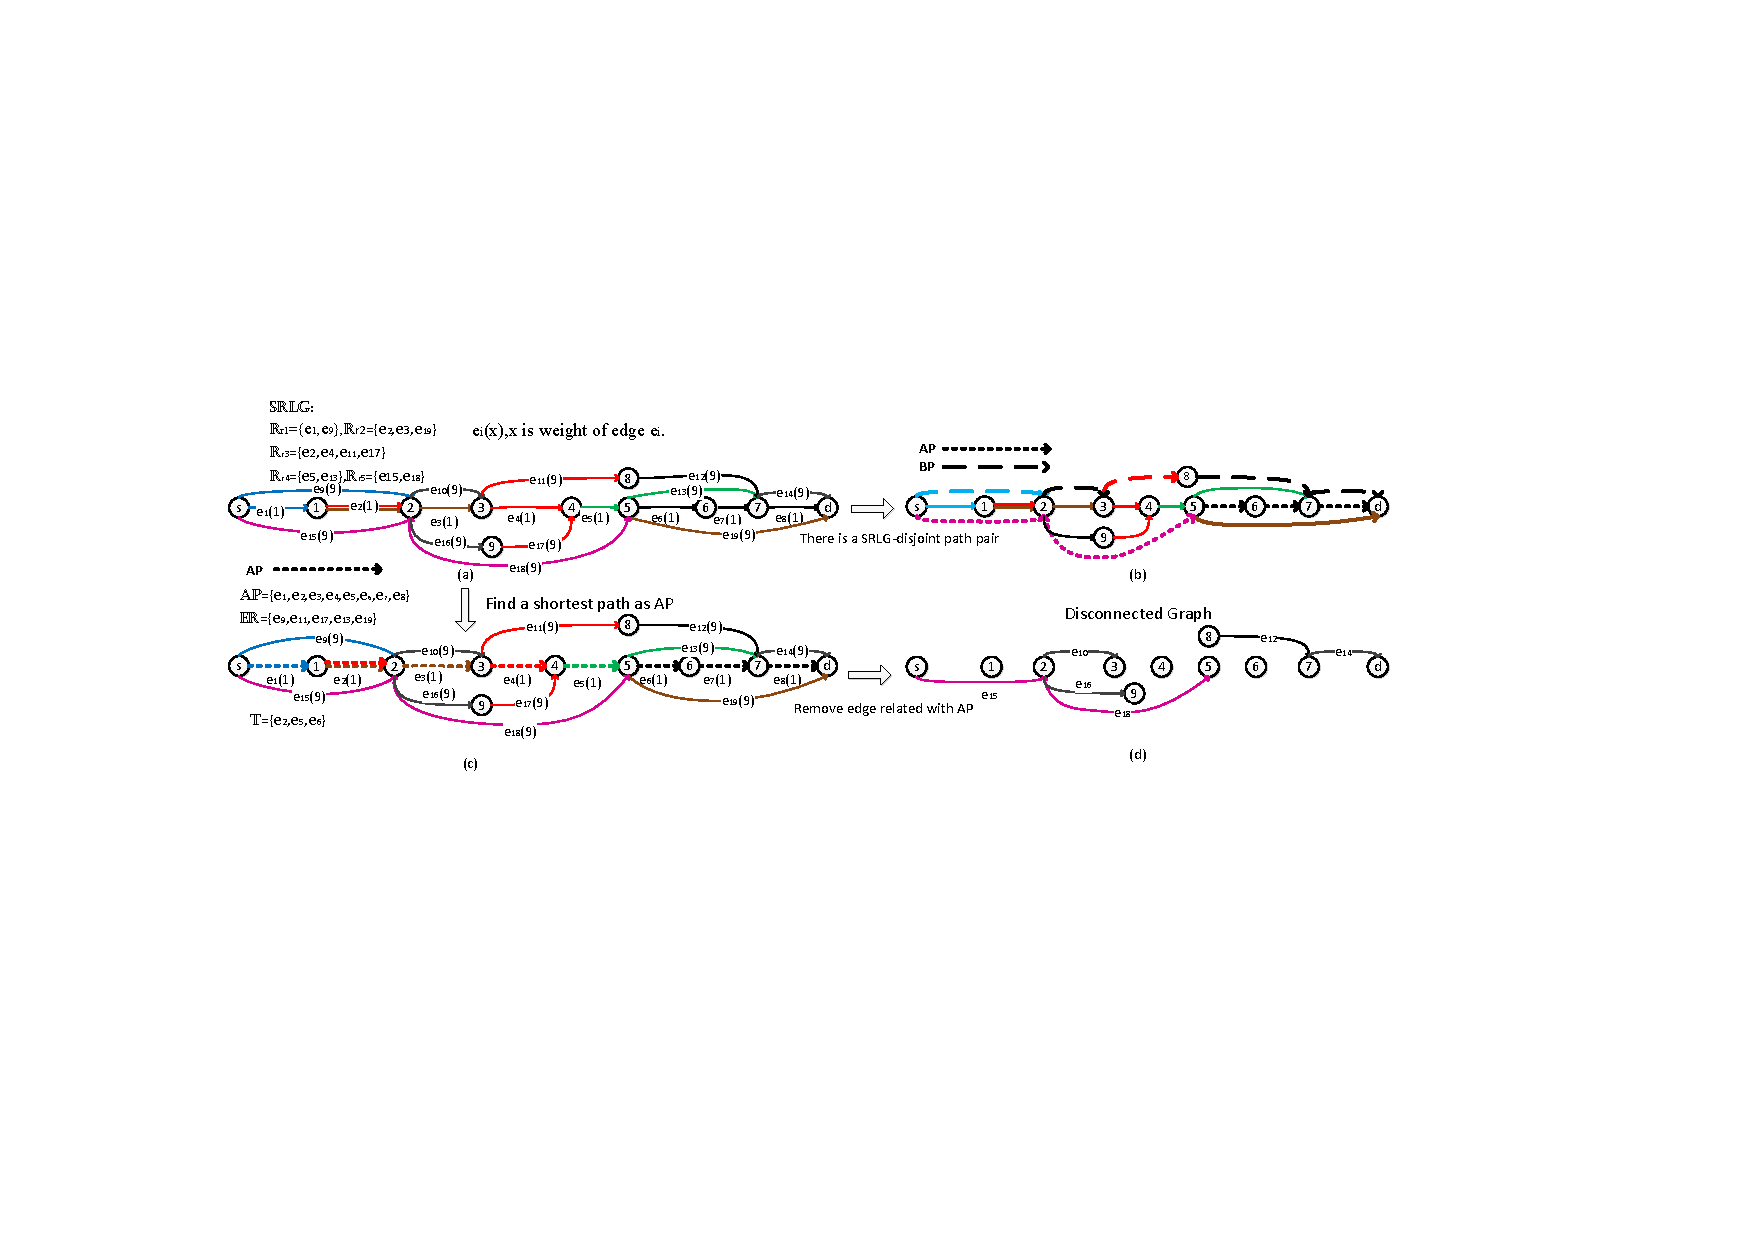
\includegraphics[width=7.2in]{figures/CompositeGraph}
  \caption{(a) A graph with five SRLGs: $\mathbb{R}_{r_1}=\{e_1,e_9\}$,$\mathbb{R}_{r_2}=\{e_2,e_3,e_{19}\}$,$\mathbb{R}_{r_3}=\{e_2,e_4,e_{11},e_{17}\}$,$\mathbb{R}_{r_4}=\{e_5,e_{13}\}$,$\mathbb{R}_{r_5}=\{e_{15},e_{18}\}$. (b)AP and BP in the graph. (c) The shortest weight path AP in the graph. $\mathbb{AP}=\{e_1,e_2,e_3,e_4,e_5,e_6,e_7,e_8\}$, $\mathbb{\mathbb{ER}}=\{e_9,e_{11},e_{17},e_{13},e_{19}\}$. (d)  Graph after deleting the links in $\mathbb{AP}$ and ${\mathbb{ER}}$. }
  \label{fig:CompositeGraph}
\end{figure*}

\section{原有算法概述}
共享风险链接组(SRLG)是一组链路共享相同的一个组件,该组件的故障会导致在这个组里所有链接的发生故障。就路径保护而言,尽管某些链路或者节点分离路径算法\cite{suurballe1984quick,bhandari1997optimal,li1990complexity,guo2003link,xu2004finding,beshir2011variants,guo2013finding,hu2003diverse} 已经提出来,SRLG分离路径 问题是比较棘手的,而且这些原有研究是限制在一定领域的。比如当每个SRLG只包含一条链路时,这个SRLG分离路由问题可以简化为链路分离路径问题,而通过节点分离方法(node split method)\cite{ford2015flows}节点分离路径问题可以转化为链路分离路径问题。因为SRLG组通常包括的链路超过一条并且网络中的链路通常可以属于多个SRLG组里,以至于求一对SRLG 分离路径问题比求一对链路或者节点分离路径问题要困难得多。

为了解决SRLG分离路径问题,一种可能的方法是0-1整数线性规划(ILP)\cite{hu2003diverse},通过分支限界法(branch-and-bound)来搜索来选择最优的主路径和备份路径。该方法时间复杂度高,不适用于大型网络。为了降低算法的复杂度,基于APF的启发式算法\cite{oki2002disjoint,li2002fiber,eppstein1998finding}能够求Min-Min SRLG分离路径问题的近似最优解。首先使用Dijkstra算法(或任何其他最短路径算法)求出主路径,求主路径时不考虑其相应的备用路径情况,在删除AP沿线的链路并且与AP共风险的节点和链路后,再利用最短路算法求的备用路径。

然而,使用APF启发式算法的有一个主要缺陷,一旦求得路径AP后也可能无法找到相对的SRLG分离路径BP,即使网络中确实存在一对分离路径。这就是所谓的“陷阱”问题,即使稠密网络中\cite{laborczi2001solving}这也是可能发生,在一个稀疏连接的网络中当然不能被忽略。陷阱有两种:不可避免的陷阱和可避免的陷阱。不可避免的陷阱是受拓扑约束的,任何算法都无法解决。如果网络不是2-边连通度的,则没有算法可以保证在拓扑中存在两个SRLG分离路径。另一方面,当两个节点之间存在SRLG分离路径对,但由于路由算法的缺陷而找不到时,就会出现一个可避免的陷阱。在本章中只考虑了可避免的陷阱。

对简单的APF算法的扩展,提出了KSP(K-最短路径)算法来处理节点/链路分离路径的陷阱问题。虽然它是处理陷阱问题最有效的算法之一,但它在大型网络中的性能受到影响,因为KSP 可能会涉及多路径搜索测试(K测试),直到它找到分离路径。当前候选的路径AP遇到陷阱问题后,仅根据路径长度选择下一个要测试的候选AP,而不考虑当前候选AP的那条链路(或那些链路)导致查找分离路径BP失败。因此,为了找到一对分离路径对,需要对大量的路径进行测试,这就引入了KSP算法中与K相关的时间复杂度。对于遇到陷阱问题的AP,我们应用从AP 路径导出的SRLG冲突链路集来指导将来的AP路径测试。这在很大程度上有助于减少寻找替代路径的时间复杂度。

其它SRLG分离路径算法\cite{rostami2012msdp,rostami2007cose,datta2008graph,xu2003new,todimala2004imsh},搜索最大SRLG分离路径对,并且路径间共享最小数目的公共链路。由于AP 和BP 可能具有相同的风险资源组,通过这种方法找到的解决方案是不可靠的。我们的算法目标是寻找完全SRLG分离路径。Xu\cite{xu2003trap}试图找到完全SRLG 分离路径。但他的算法减少了问题的搜索空间,加快了路径搜索的速度。然而,它可能会以较大的代价返回路径,因为在削减后的空间可能会失去最优解。相反,为了大大加快搜索过程,我们利用SRLG冲突链接集将原问题划分为多个子问题,这些子问题可以并行执行。因此,我们的算法可以运行得更快,返回主路径成本非常低。

Datta\cite{datta2008graph}提出方法是将SRLG分离路径问题转化为链路分离路径问题,然后利用链路分离路径算法来解决。然而,只有特殊的SRLG模式(例如,星型)可以
将其转换为链路分离,这样就限制了该算法的广泛应用。当AP遇到陷阱问题时,CoSE\cite{rostami2007cose}算法试图找到一个SRLG集合,任何AP路径包含了这个SRLG集合里的所有SRLG,则必定找不到任何的与其对应的SRLG分离路径BP。CoSE 首先通过多轮搜索查找多个AP共享的SRLG,并且组成一个SRLG集合,然后根据SRLG集合来划分原始问题以搜索SRLG分离路径对。而不使用SRLG 中链路之间共享风险的特性,CoSE方法的这种穷尽搜索需要非常高的计算开销。



\section{整数规划形式化}
\section{时间复杂度}
\begin{theorem}
\label{le:lemma1}
    Min-Min SRLG-分离路径问题是 NP-complete.
\end{theorem}
\begin{proof}
根据\cite{bhatia2006finding},Min-Min链路分离路径问题是NP-complete 的。Min-Min链路分离路径问题是Min-Min SRLG-分离路径问题的子问题。设
Min-Min SRLG分离路径问题的复杂性为C(A),则NP-complete的$\leq$C(A).

为了求Min-Min SRLG分离路径问题的时间复杂度,我们首先假设了一个问题B(问题B的复杂性表示为C(B)),当找到两条的SRLG分离路径并且路径较小的路径其权重小于或等于M(M是大于零整数数)。Min-mim SRLG分离路径问题A与问题B等价,我们知道M必须大于零并且小于$\sum\limits_{e_i\in \mathbb{E}}w_{e_i}$。例如,我们假设0≤M≤10和m=6是最优解,通过经典的二分法(binary search method)时间复杂度为O(log(N)),如图.\ref{fig:binarySearch}所示,通过二分法我们得到了两条分离的路径,较小的路径其权重为m,因此问题A与 问题B等价。
\begin{figure}[htp]
  \centering
  % Requires \usepackage{graphicx}
  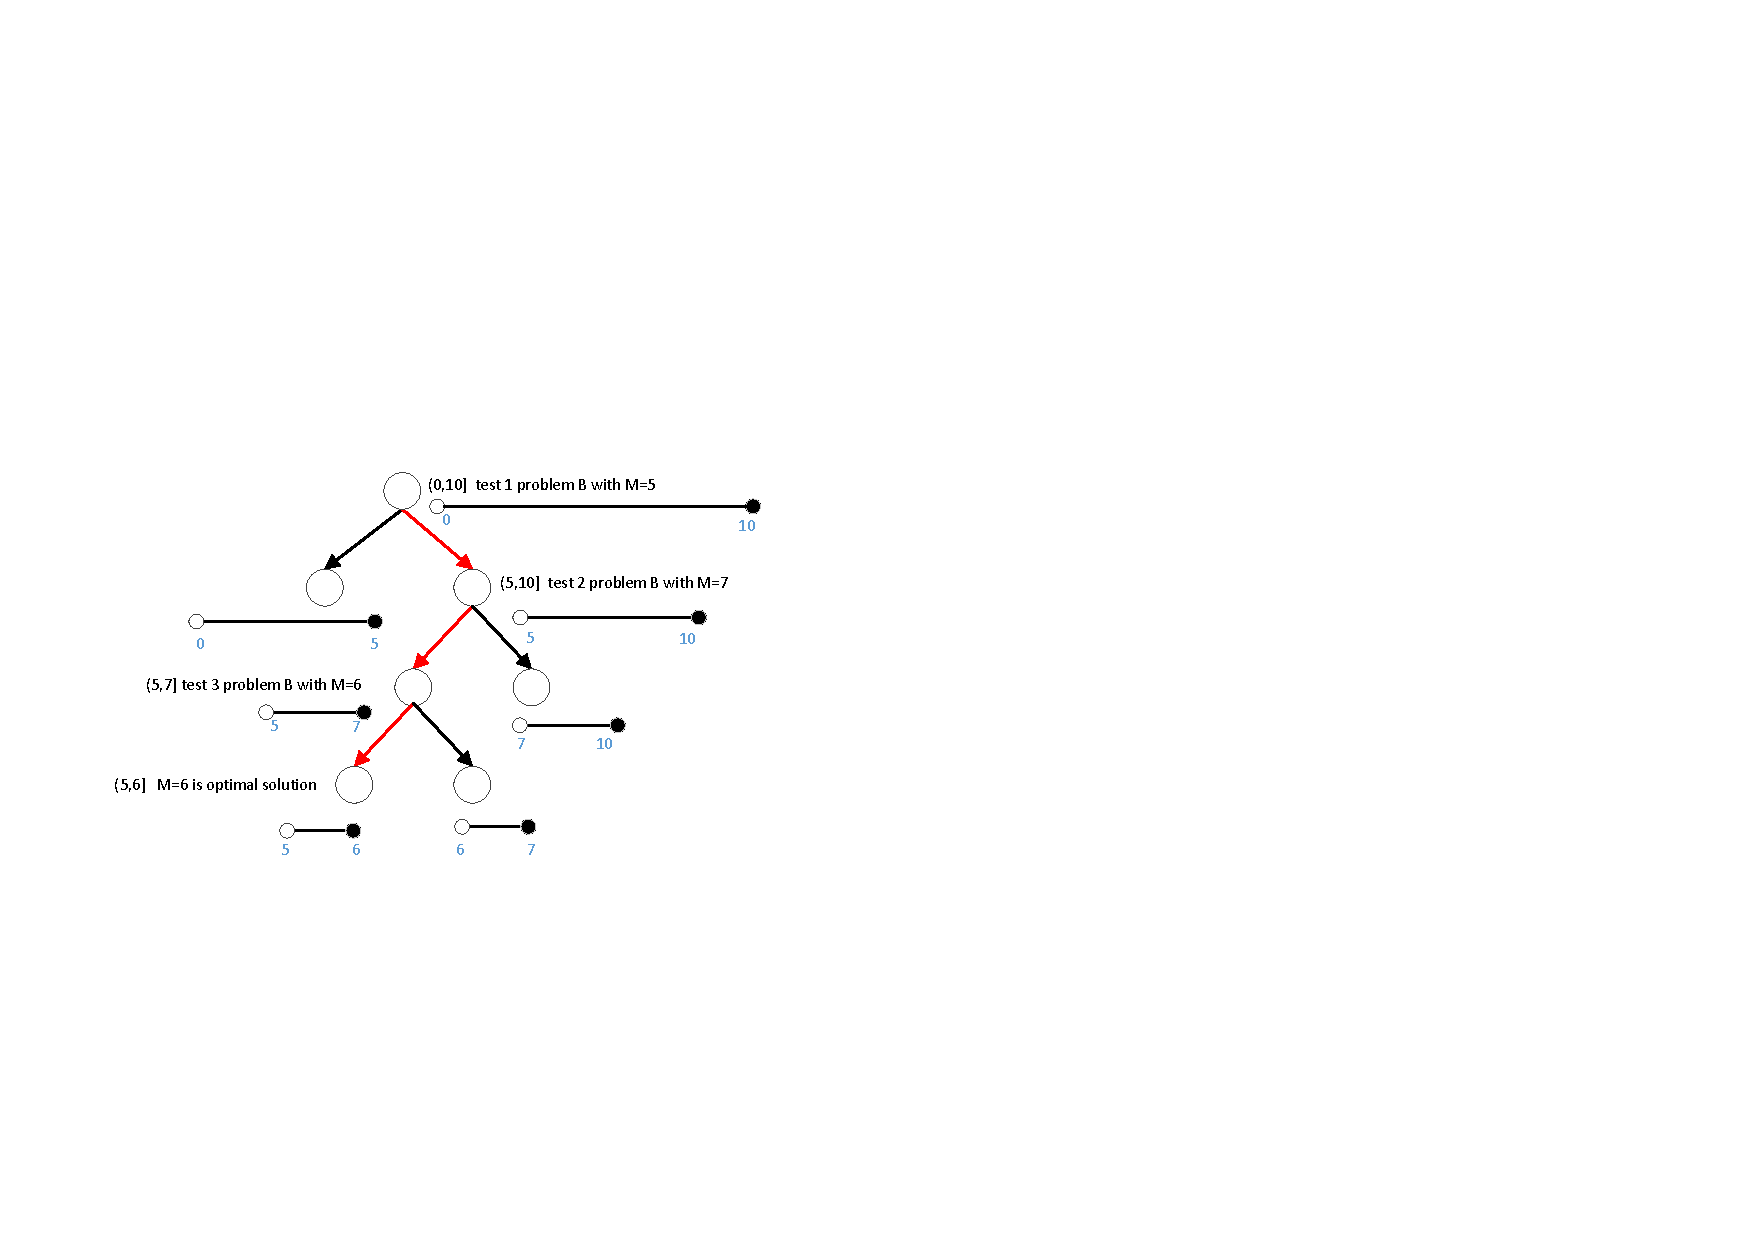
\includegraphics[width=3.0in]{figures/binarySearch}
  \caption{Request optimal solution M through Binary search method }
  \label{fig:binarySearch}
\end{figure}
假设程序X在输入问题B时,如果问题B没有解,则程序Y立即停止,否则程序B继续执行并获得问题B的解,因此问题B可以归结为NP-hard问题。因此C(B)$\leq$NP-hard。

此外,给定任意两条路径,很容易在多项式时间内判别这两条路径是否为SRLG 分离路径,较小的路径其权重小于或等于M,从而使得C(B)$\leq$NP-complete。当B的复杂度等于A时,我们有C(A)=C(B)$\leq$NP-complete。因此,A=NP-complete。
\end{proof}
\section{陷阱问题}
基于APF的启发式算法可能会陷入“陷阱”问题。也就是说,当一个AP被确定时,即使网络中确实存在一对分离路径对,它也可能无法找到SRLG分离的BP路径。图.\ref{fig:CompositeGraph}.(c),(d)说明了陷阱问题。虚线表示一个AP,其链路集为$\mathbb{AP}=\{e_1,e_2,e_3$ $,e_4,e_5,e_6,e_7,e_8\}$。在删除AP上的链路和与AP共享风险的链路后,图.\ref{fig:CompositeGraph}.(d) 所示的不存在从s到d的路径,因此找不到BP。

虽然KSP算法被认为是解决陷阱问题的有效算法,但它可能面临着效率低下的问题。在这个图.\ref{fig:KSPproblem}中,假设$e_1, e_2, e_3, e_4$的链路权重比其他链路大得多。此外,在$e_1, e_2, e_3, e_4$中,$e_1$ 和$e_2$的链接权重远小于$e_3$,$e_4$。然后,在KSP算法多次找从s到d的K短路时,总是包含$e_1,e_2$(虚线表示)。则最短AP 总会遇到陷阱问题,因为$e_1$和$e_4$ 具有相同的风险,因此无法找到BP。为了避免陷阱问题,必须将K设为一个大值,这给KSP带来了很高的时间复杂度。
\begin{figure}[htbp]
\centering
% Requires \usepackage{graphicx}
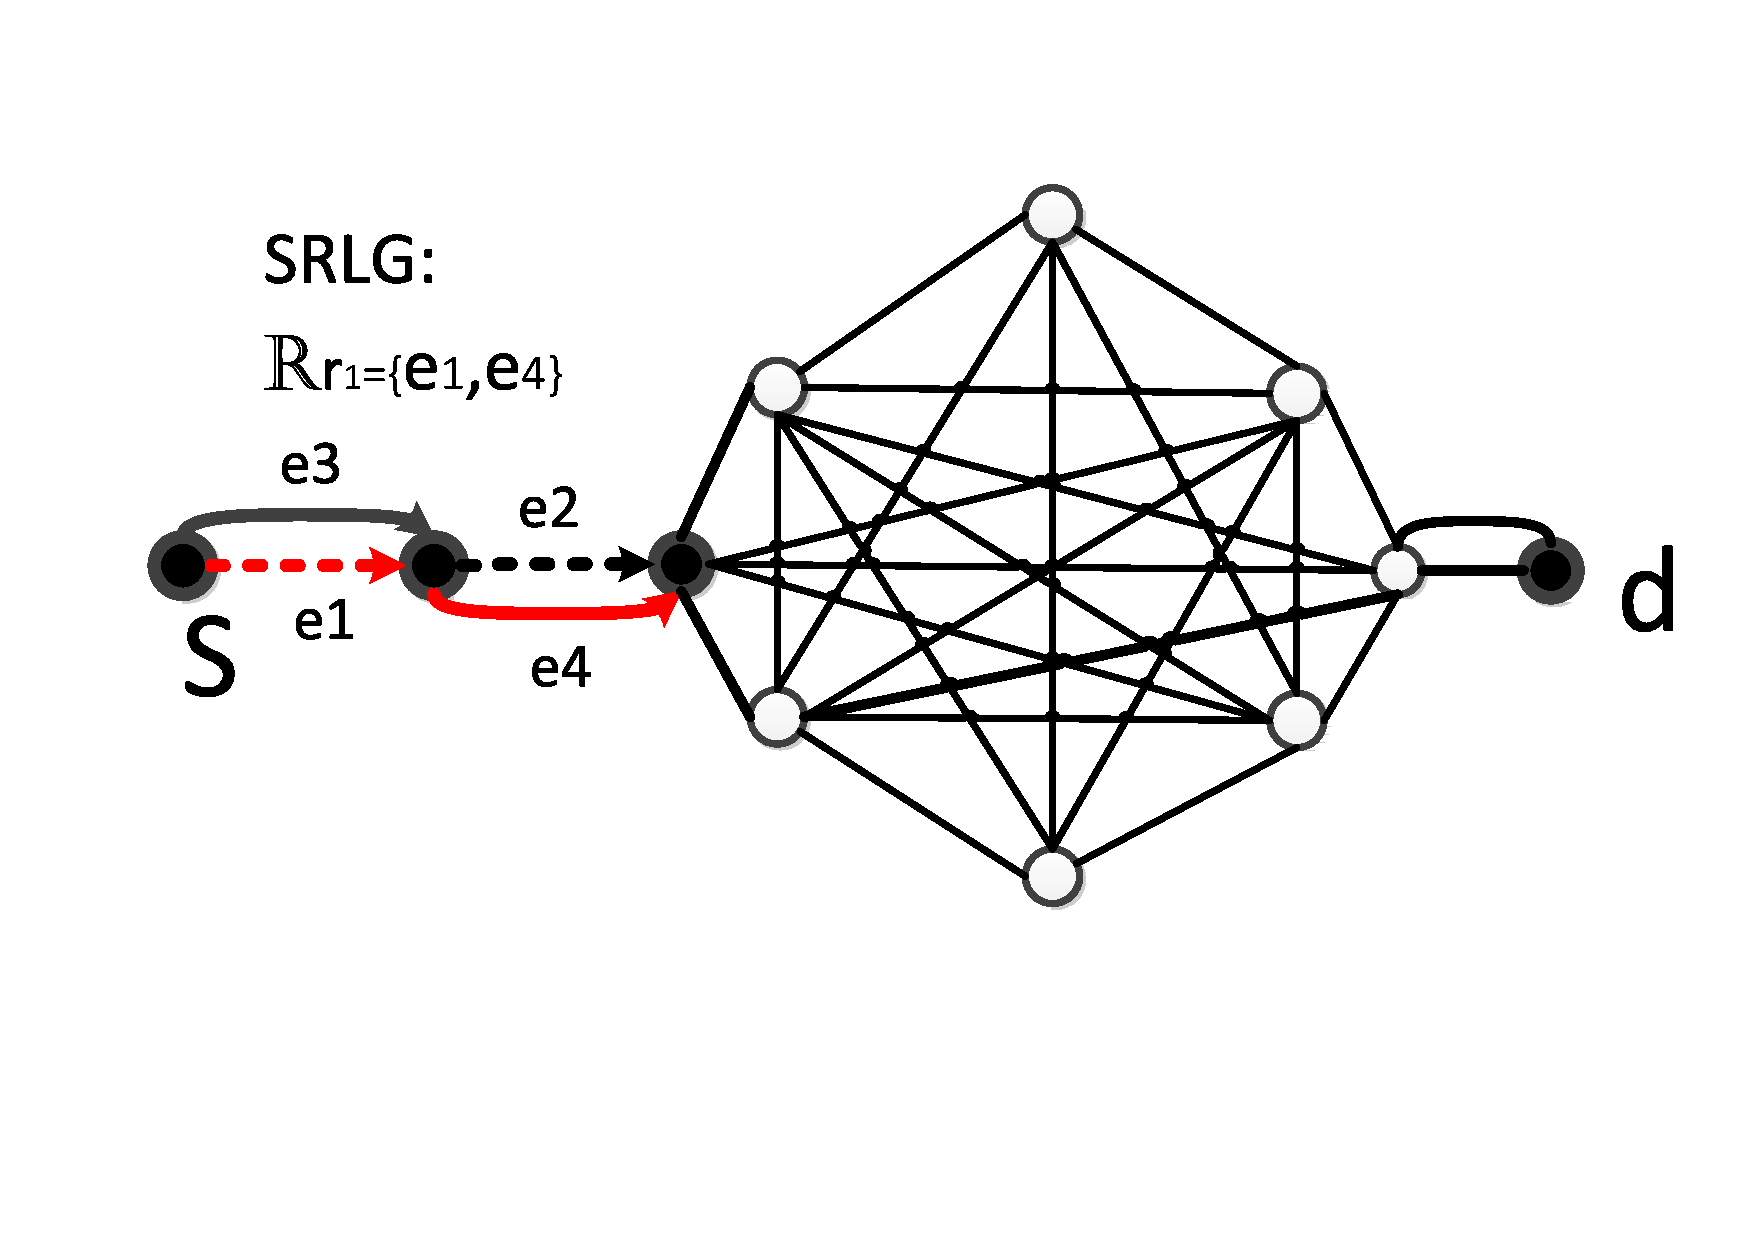
\includegraphics[width=2.8in]{figures/KSPproblem}
  \caption{An example to illustrate the inefficiency of KSP}
  \label{fig:KSPproblem}
\end{figure}


\section{分而治之的快速共享风险链路组分离路径算法}
当一个陷阱问题发生,并且对于给定的AP没有SRLG分离路径BP时,AP中可能存在一个子链路集,这样任何通过这个链路集里所有的这些“问题”链路的AP都不能找到一个SRLG分离BP。 我们称之为\textbf{SRLG冲突链路集}。与KSP不同,当最短AP遇到陷阱问题时,我们将通过两个主要步骤来解决这个问题。在图.\ref{fig:KSPproblem}的例子中,我们将首先找到图.\ref{fig:KSPproblem}中的SRLG冲突链路p集合,然后应用分而治之算法将原问题划分为两个子问题$\mathcal{P}(\emptyset,\{e_1\})$和 $\mathcal{P}(\{e_1\},\{e_2\})$。 这两个子问题可以在多核CPU平台上并行执行,快速得到SRLG分离路径对。
\subsection{分而治之}
在得到SRLG冲突链路集后,设计了一种分而治之的算法,将原Min-Min SRLG不相交路由问题划分为多个子问题,并行执行,加快求SRLG分离路径对的过程。

为了便于问题划分,我们首先用定义两个不相交的链接集和$\mathbb{I}$和$\mathbb{O}$,其中我被称$\mathbb{I}$为包含集集合,$\mathbb{O}$称为排除集集合。由$\mathcal{P}({\mathbb{I},\mathbb{O}})$表示的Min-Min SRLG- 分离问题,用于寻找一对AP和BP,其中AP是所有可能的AP中最短的,其中路径$AP$必须经过$\mathbb{I}$集合里的所有链路和不经过$\mathbb{O}$集合里的所有链路

最初,让$\mathbb{I}=\emptyset$ 和 ${\mathbb{O}}=\emptyset$,原来的Min-Min SRLG分离路径对问题可以用$\mathcal{P}(\emptyset,\emptyset)$表示。给定SRLG冲突链路集$\mathbb{T}=\{{e_1},{e_2}, \cdots ,{e_{\left| \mathbb{T} \right|}}\}$,原问题$\mathcal{P}(\emptyset,\emptyset)$可按以下步骤划分。

\begin{enumerate}
  \item 首先,$\mathcal{P}(\emptyset,\emptyset)$能被划分成两个子问题$\mathcal{P}(\emptyset,\{e_1\})$ 和 $\mathcal{P}(\{e_1\},\emptyset)$。
  \item 类似,$\mathcal{P}(\emptyset,\{e_1\})$能被划分成两个子问题 $\mathcal{P}(\{e_1,e_2\},\emptyset)$ 和 $\mathcal{P}(\{e_1\},\{e_2\})$。
  \item 这个划分步骤持续直到步骤$|\mathbb{T}|$,问题$\mathcal{P}(\{e_1,e_2,\cdots ,{e_{\left| \mathbb{T} \right|-1}}\},\emptyset)$ 进一步的拆分成两个子问题$\mathcal{P}(\{e_1,e_2,\cdots ,{e_{\left| \mathbb{T} \right|-1}}, {e_{\left| \mathbb{T} \right|}}\},\emptyset)$ 和 $\mathcal{P}(\{e_1,e_2,\cdots ,{e_{\left| \mathbb{T} \right|-1}}\},{e_{\left| \mathbb{T} \right|}})$。注意到,子问题$\mathcal{P}(\{e_1,e_2,\cdots ,{e_{\left| \mathbb{T} \right|-1}}, {e_{\left| \mathbb{T} \right|}}\},\emptyset)$是无解的。
\end{enumerate}



除了子问题$\mathcal{P}(\{e_1,e_2,\cdots ,{e_{\left| \mathbb{T} \right|}}\},\emptyset)$外,我们将试图求其它每个子问题的最优解。然后选择最好的路径对(即最短路径对)。作为原问题$\mathcal{P}(\emptyset,\emptyset)$的最终(最优)解。如果这些子问题都没有解,则我们可以得出原问题没有任何解,因为我们子问题包括了所有的可能的分离路径对。

就时间复杂性而言,解决子问题所需的时间比原来的问题应该花费的更少。因为一条链路(来自集合$\mathbb{T}$)将在计算AP的路径时被去除,这也确保了不同的AP路径将被测试且是否存在一个SRLG分离BP路径。

当遇到陷阱问题时,我们的解决方案将划分原来的问题,并测试每个子问题以寻找到最终的解。在我们的分而治之方法中,子问题是由SRLG冲突链路集而得,而这个SRLG冲突链路集适是当AP路径遇到陷阱问题生成的。与现有的算法相比较,该算法在不考虑现有结果和问题的情况下,可以在很大程度上降低算法的计算量。对于图.\ref{fig:DividedConquer}中的例子所示,SRLG冲突链接集是$\mathbb{T}=\{e_2,e_5,e_6\}$。拆分过程过程如图.\ref{fig:DividedConquer}所示。根据SRLG冲突链路集,我们应该测试总共3个子问题${{\mathcal{P}}(\{ e_2,e_5\} ,\{ e_6\} )}$, ${{\mathcal{P}}(\{ e_2\} ,\{ e_5\} )}$ 和 ${{\mathcal{P}}(\emptyset ,\{ e_2\} )}$,其中选择AP路径权重最低的最优子问题作为原问题$\mathcal{P}(\emptyset,\emptyset)$最终的(最优)解。

注意,我们不需要解决子问题${{\mathcal{P}}(\{ e_2,e_5\}, \emptyset)}$ 和 ${{\mathcal{P}}(\{ e_2\},\emptyset )}$,因为它们的解已经包含在其它的子问题中。第一个解空间由两个子问题${{\mathcal P}(\{ e_2,e_5,e_6\} ,\emptyset )}$ 和 ${{\mathcal P}(\{ e_2,e_5\} ,\{ e_6\} )}$组成。由于SRLG冲突链接集为$\mathbb{T}=\{e_2,e_5,e_6\}$,显然,子问题${{\mathcal P}(\{ e_2,e_5,e_6\} ,\emptyset )}$是没有解的。因此,${{\mathcal P}(\{ e_2,e_5\} ,\{ e_6\} )}$的解空间等于${{\mathcal{P}}(\{ e_2, e_5\}, \emptyset)}$的解空间。同样,${{\mathcal{P}}(\{ e_2\},\emptyset )}$的解空间包括${{\mathcal{P}}(\{ e_2\} \{ e_5\}, \emptyset)}$  和 ${{\mathcal{P}}(\{ e_2\} ,\{ e_5\} )}$的解空间。
\begin{figure}[htbp]
\small{
\begin{equation*}
{\mathcal P}(\emptyset ,\emptyset )\left\{ {\begin{array}{*{20}{l}}
{{\mathcal P}(\{ e_2\} ,\emptyset )\left\{ {\begin{array}{*{20}{l}}
{{\mathcal P}(\{ e_2,e_5\} ,\emptyset )\left\{ {\begin{array}{*{20}{l}}
{{\mathcal P}(\{ e_2,e_5,e_6\} ,\emptyset )}\\
{\boxed{{\mathcal P}(\{ e_2,e_5\} ,\{ e_6\} )}}
\end{array}} \right.}\\
{\boxed{{\mathcal P}(\{ e_2\} ,\{ e_5\} )}}
\end{array}} \right.}\\
{\boxed{{\mathcal P}(\emptyset ,\{ e_2\} )}}
\end{array}} \right.
\end{equation*}
}
\caption{Example to illustrate divide-and-conquer solution}
\label{fig:DividedConquer}
\end{figure}




\subsection{SRLG冲突链路集合}
在本节中,我将描述了如何找到一个SRLG冲突链路集合,当在网络$G$中给定一个AP路径并且没有SRLG分离的BP路径。
\subsubsection{通过新奇的边容量设置准则构造一个新的图$G^*$}
如\ref{subsubsec:maxFlow}节介绍的,如果在图G中去除所有在边割集$\mathbb{\mathbb{L}}_{\Phi}$的所有边,则$|f| = 0$。也就是说,不存在任何流能从$s$到$d$。在本文中,我们试图基于割集的概念找到SRLG冲突链路集合。如果AP从s到d流通,经过的链路与割集$\mathbb{\mathbb{L}}_{\Phi}$共享风险,则找不到任何与其对应的SRLG分离路径BP,因为没有一条在割集中的链路可以被BP选择。

基于割集上基础上为了找到SRLG 冲突链路集,我们构造了一个新的图$G^*$ ,如下所示.
\begin{enumerate}
  \item $G^*$与$G$的节点和链路结构一样
  \item 跟每条链路$e_i$相关的链路权重$w_{e_i}$是跟其相对应图$G$中边的权重一样的。
  \item 我们使用以下准则设置每条边$e_i \in \mathbb{E}$相关的容量$c_{e_i}$
\end{enumerate}
 \begin{equation}
c_{e_i} = \left\{ {\begin{array}{*{20}{c}}
   1 & {e_i{\rm{ }} \in {\rm{ \mathbb{AP}}}}  \\
   {\left| \mathbb{AP} \right|+1} & {e_i{\rm{ }} \in {\rm{ \mathbb{E}}}{{\rm{\mathbb{R}}}}}  \\
   {\left| {{\rm\mathbb{AP}}} \right| + \left( {\left| {{\rm\mathbb{AP}}} \right| + 1} \right)\times \left| {{\rm{\mathbb{E}}}{{\rm{\mathbb{R}}}}} \right| + 1} & {otherwise}  \\
\end{array}} \right.
\label{eq:capacity principle}
\end{equation}
$\mathbb{AP}$指在图$G$中较小权重路径$AP$上所有链路的集合,和$\mathbb{\mathbb{ER}}$指不属于路径$AP$上的边但是与路径$AP$上的边共享风险的链路集合。

在图.\ref{fig:CompositeGraph}(c)所示,路径$AP$的边集合$\mathbb{AP}=\{e_1,e_2,e_3,e_4$
$,e_5,e_6,e_7,e_8\}$, $\mathbb{\mathbb{ER}}=\{e_9,e_{11},e_{17},e_{13},e_{19}\}$。$|\mathbb{AP}|=8$, $|\mathbb{\mathbb{ER}}|=5$, $|\mathbb{AP}|+1=9$ 和 ${\left| {{\rm{\mathbb{AP}}}} \right| + \left( {\left| {{\rm{\mathbb{AP}}}} \right| + 1} \right)\times \left| {{\rm{\mathbb{E}}}{{\rm{\mathbb{R}}}}} \right| + 1}=54$. 我们产生一个新图$G^*$如图.\ref{fig:FlowStarGraph}所示, 在图$G^*$中边的容量是根据公式.(\ref{eq:capacity principle})所设置.

\begin{figure}[tp]
  \centering
  % Requires \usepackage{graphicx}
  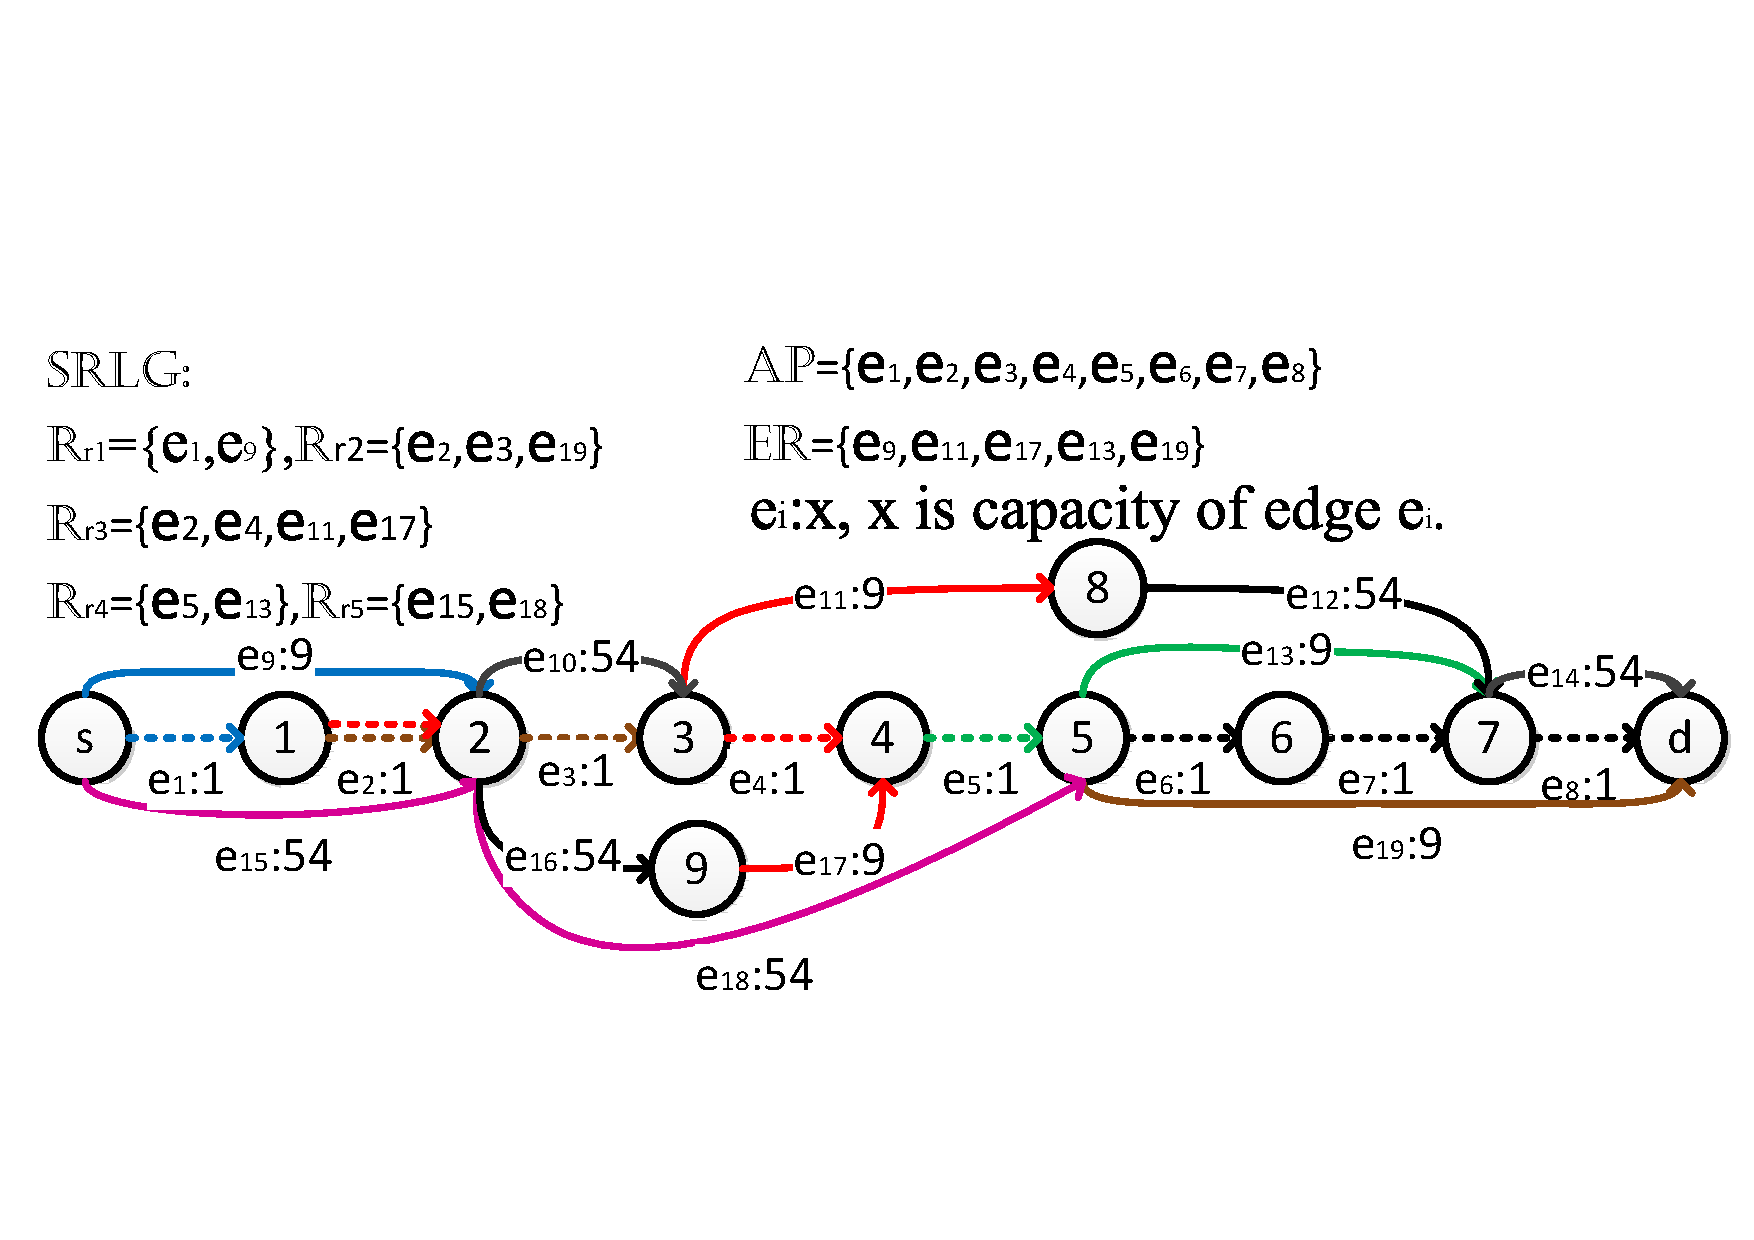
\includegraphics[width=3.6in]{figures/FlowStarGraph}
  \caption{New Graph $G^*$}\label{fig:FlowStarGraph}
\end{figure}

\subsubsection{新图$G^*$中最小割集的性质}
最大流最小割定理指出,在网络中,从源节点$s$到目的节点$d$最大流值等于最小边割集的总容量,即最小的链路总容量,如果删除最小边割集上的边,将断开目的节点$d$与源节点$s$的连通。 我们的算法基于图的最小割集的链路集来求得最小SRLG 冲突链路集。

我们将首先展示我们重建新图$G^*$的一些优良特性为求得最小SRLG冲突链路集。

\begin{lemma}
\label{le:lemma1}
    在图$G^*$任何从$s$到$d$的路径必须经过一条边在边集合 $\mathbb{AP}$ 或者 $\mathbb{\mathbb{ER}}$中。
    %note:draw a picture to describe the proof
\end{lemma}
\begin{proof}
我们用矛盾的方法证明这条引理。假设对于某条路径AP,有另一条路径从$s$到$d$在图$G^*$中不与AP共享风险,即这条路径不通过$\mathbb{AP}$ 或者 $\mathbb{\mathbb{ER}}$的任何一条链路。我们可以很容易得出这样的结论,这条路径是与路径AP对应的SRLG分离路径BP。这与AP没有对应的SRLG分离路径的说法相矛盾。
\end{proof}

\begin{lemma}
\label{le:lemma2}
    图$G^*$的任何一条最大流的流值是最多为$|\mathbb{AP}|+(|\mathbb{AP}|+1)\times|\mathbb{\mathbb{ER}}|$。
\end{lemma}
\begin{proof}
假设$G^*$的最大流f为$|f|=k$。在$G^*$中,f可以被划分为k个从s到d的1单元流。根据引理.\ref{le:lemma1},这些1单位流中的每一个都必须通过通过$\mathbb{AP}$ 或者 $\mathbb{\mathbb{ER}}$的至少一个链路。请注意,$\mathbb{AP}$ 或者 $\mathbb{\mathbb{ER}}$ 中链路的容量分别为1或者$|\mathbb{AP}|$+1。根据$\mathbb{AP}$ 和 $\mathbb{\mathbb{ER}}$中链路的容量设置,因为$\mathbb{AP}$中的链路只能承载1单位流量,而在ER中,一条链路在$\mathbb{ER}$中能最多承载$|\mathbb{AP}|$+1单位流量.因此,最多只能有$|\mathbb{AP}|+ (|\mathbb{AP}|+1)\times|\mathbb{\mathbb{ER}}|$个从s到d的单位流量。
\end{proof}

\begin{lemma}
\label{le:lemma3}
    图$G^*$的最小割$\Phi$的边割集$\mathbb{L}_{\Phi}$所有链路都在$\mathbb{AP}$ 或者$\mathbb{\mathbb{ER}}$中。
\end{lemma}

\begin{proof}
根据最大流最小切定理,$c(\Phi)$表示的最小切割$\Phi$的的容量,其应该等于最大流量值,根据引理 \ref{le:lemma2}最大流量最多为$|\mathbb{AP}|+ |\mathbb{ER}|\times (|\mathbb{AP}|+1)$。 根据容量设定原则如公式\ref{eq:capacity principle}所示,一条链路既不在$\mathbb{AP}$ 也不在 $\mathbb{ER}$ ($e_i \notin \mathbb{AP}$ 和 $e_i \notin \mathbb{ER}$), 这条链路的容量为 $c_{e_i} = \left| {{\rm\mathbb{AP}}} \right| + \left( {\left| {{\rm\mathbb{AP}}} \right| + 1} \right)\times \left| {{\rm{\mathbb{E}}}{{\rm{\mathbb{R}}}}} \right| + 1$, 这条链路是大于$|\mathbb{AP}|+(|\mathbb{AP}|+1)\times |\mathbb{ER}|$. 因此,这条链路不可能在$\mathbb{L}_{\Phi}$中. 因此,割集$\mathbb{L}_{\Phi}$中的所有链路都必须属于边集合$\mathbb{AP}$ 或者 $\mathbb{ER}$。
\end{proof}


\begin{theorem}
    如果在图$G$中一个单元流阻塞了全部边割集$\mathbb{L}_{\Phi}$的所有边,则在原图中不会存在任何流经过这个图的割。
\label{th:block flow}
\end{theorem}


\begin{proof}
    如果在图$G$中一个单元流阻塞了全部边割集$\mathbb{L}_{\Phi}$的所有边,则在原图中没有流能使用边割集$\mathbb{L}_{\Phi}$ 里的边和没有任何流能经过这个图的割。
\end{proof}
定理\ref{th:block flow}提供了找到SRLG冲突链路集的可能性。即当AP路径遇到陷阱问题时,我们找到$\mathbb{AP}$路径边集的子集能够阻塞国有在边割集$\mathbb{L}_{\Phi}$的所有边,和这个子集即SRLG冲突链路集。当一条路径包含SRLG冲突链路集里的所有边,则没有任何流能经过割集$\Phi$,因此没有与其对应的SRLG分离路径BP。

\subsubsection{SRLG冲突链路集的集合覆盖问题}
虽然AP路径上的所有链接一起构成了SRLG冲突链路集,我们感兴趣的是尽量规模较小的SRLG冲突链路集,SRLG冲突链路集的大小确定分离成的子问题规模。

根据定理\ref{th:block flow},最小SRLG冲突链路集问题可以描述为:查找AP 链路集上的最小链路子集,这些链路可以阻塞边割集$\mathbb{L}_{\Phi}$。

对于任何链路$e_i$,$\mathbb{SR}_{e_i}$表示与链路$e_i$共享风险的链接集。显然,$\mathbb{SR}_{e_i}$包括$e_i$本身和所有包含链路$e_i$风险贡献链路组SRLG集合的所有边。例如,如图\ref{fig:MinCutStarGraph}所示,$e_i$ 是在两个SRLG中$\mathbb{R}_{r_2}=\{e_2,e_3,e_{19}\}$, $\mathbb{R}_{r_3}=\{e_2,e_4,e_{11},e_{17}\}$,因此, $\mathbb{SR}_{e_2}=\{e_2,e_3,e_{19},e_4,e_{11},e_{17}\}$。

对每条在AP上的路径$e_i$,我们定义每条边的cut-block-link集合为${\mathbb{B}_{{e_i}}} = \mathbb{SR}_{{e_i}} \cap \mathbb{L}_{\Phi}$,这个集合是边割集$\mathbb{L}_{\Phi}$的子集,能通过$e_i$而堵塞这个集合的所有边。

因此,最小SRLG冲突链路集问题可以定义为一个集合覆盖问题:给定$\mathbb{AP}$(路径AP上的链路集合)、边割集$\mathbb{L}_{\Phi}$和cut-block-link集合${\mathbb{B}_{{e_1}}},{\mathbb{B}_{{e_2}}}, \cdots ,{\mathbb{B}_{{e_{|\mathbb{AP}|}}}}$。我们求出最小cut-block-link集合集,其交集是边割集$\mathbb{L}_{\Phi}$,即最小规模的$\mathbb{T} \subseteq \{e_i| e_i\in \mathbb{AP}\}$ 以至于 ${ \cup_{e_i \in \mathbb{T}}}{\mathbb{B}_{e_i}} = \mathbb{L}_{\Phi}$。


\begin{figure*}[htbp]
  \centering
  % Requires \usepackage{graphicx}
  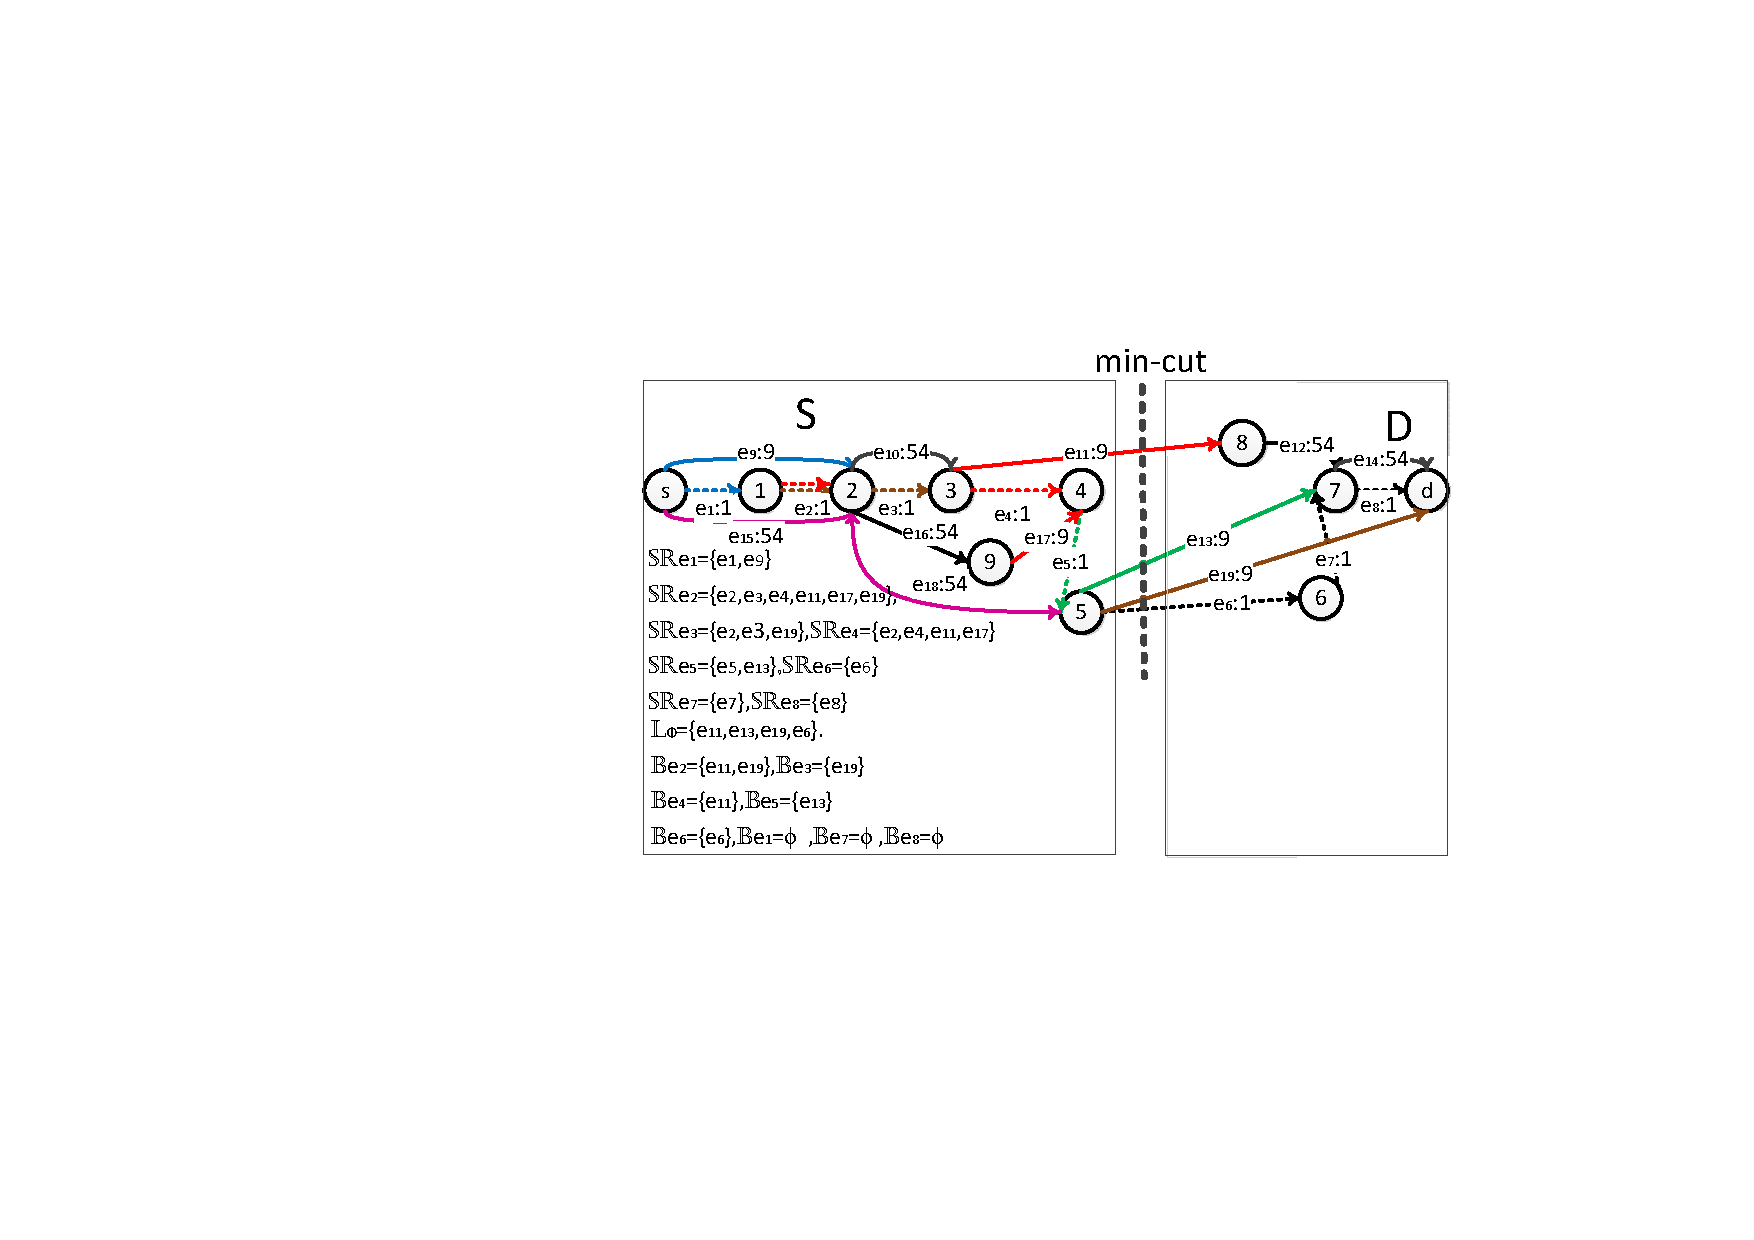
\includegraphics[width=3.8in]{figures/MinCutStarGraph}
  \caption{Min cut of the network graph, $\mathbb{SR}_{e_1}=\{e_1, e_9\},\mathbb{SR}_{e_2}=\{e_2,e_3,e_4, e_{11},e_{17},e_{19}\},\mathbb{SR}_{e_3}=\{e_2,e_3, e_{19}\},\mathbb{SR}_{e_4}=\{e_2,e_4, e_{11},e_{17}\},\mathbb{SR}_{e_5}=\{e_5, e_{13}\},\mathbb{SR}_{e_6}=\{e_6\},\mathbb{SR}_{e_7}=\{e_7\} $ and $\mathbb{SR}_{e_8}=\{e_8\}$. $\mathbb{L}_{\Phi}=\{e_{11},e_{13},e_{19},e_{6}\}$. $\mathbb{B}_{e_1}=\emptyset,\mathbb{B}_{e_2}=\{e_{11},e_{19}\},\mathbb{B}_{e_3}=\{e_{19}\},\mathbb{B}_{e_4}=\{e_{11}\},\mathbb{B}_{e_5}=\{e_{13}\},\mathbb{B}_{e_6}=\{e_6\}$,$\mathbb{B}_{e_7}=\emptyset$ and $\mathbb{B}_{e_8}=\emptyset$.}\label{fig:MinCutStarGraph}
  \label{fig:MinCutStarGraph}
\end{figure*}

集合覆盖问题通常是一个np-hard问题。它的复杂性取决于元素的大小(表示($N$)。在我们的最小SRLG冲突链路集问题中,$n=|\mathbb{L}_{\Phi}|$,即割集$\mathbb{L}_{\Phi}$的边数。因为本文的重点不是改进集合覆盖问题算法,我们应用\cite{chvatal1979greedy}中提出的算法。在复杂度$O(log(|\mathbb{L}_{\Phi}|))$的情况下求出最小的SRLG冲突链路集,通常即使是在大规模的网络,最短的路径作为AP都没有大跳数$n=|\mathbb{L}_{\Phi}|$。因此,用集合覆盖问题来求最小值SRLG冲突链路集代价不是很大。

为了说明如何找到最小SRLG冲突链路集,我们如图\ref{fig:MinCutStarGraph}所展示了一个例子。为了求最小$\Phi(\mathbb{S},\mathbb{D})$, $\mathbb{S}=\{s, 1, 2, 3, 4, 5, 9\}$和$\mathbb{D}=\{d, 6, 7, 8\}$。边割集$\mathbb{L}_{\Phi}=\{e_{11},e_{13},e_{19},e_{6}\}$。对于AP路径上的所有链路,cut-block-link集合是:$\mathbb{B}_{e_1}=\emptyset$, $\mathbb{B}_{e_2}=\{e_{11},e_{19}\}$, $\mathbb{B}_{e_3}=\{e_{19}\}$, $\mathbb{B}_{e_4}=\{e_{11}\}$, $\mathbb{B}_{e_5}=\{e_{13}\}$, $\mathbb{B}_{e_6}=\{e_6\}$, $\mathbb{B}_{e_7}=\emptyset$ and $\mathbb{B}_{e_8}=\emptyset$。为了覆盖$\mathbb{L}_{\Phi}$,最少的cut-block-link集合是$\mathbb{B}_{e_6}=\{e_6\}$, $\mathbb{B}_{e_7}=\emptyset$ and $\mathbb{B}_{e_8}=\emptyset$。因此,最小SRLG冲突链路集是$\mathbb{T}=\{e_2, e_5, e_6 \}$。

如图\ref{fig:MinCutStarGraph}所示的例子中,虽然$|\mathbb{L}_{\Phi}|=4$,但是最小SRLG冲突链路集$|\mathbb{T}|=|\{e_2, e_5, e_6 \}|=3$是小于$|\mathbb{L}_{\Phi}|=4$。这是因为$e_2$属于$\mathbb{R}_{r_2}$和$\mathbb{R}_{r_3}$,并能阻塞在割集$\mathbb{L}_{\Phi}$中的两条链路$e_{11}$和$e_{19}$


根据SRLG的拓扑类型\cite{datta2008graph},SRLG的拓扑类型:星型类型和非星型类型。对星型类型SRLG,所有链路都从同一个节点开始或结束在同一个节点。例如,如图\ref{fig:MinCutStarGraph}所示,$e_1$和$e_9$来自相同的节点$s$,$\mathbb{R}_{r_1}$是星型SRLG。对非星型类型,并不是SRLG中的所有链路都是从相同节点开始或结束于同一节点。如图\ref{fig:MinCutStarGraph}所示,$\mathbb{R}_{r_2}$, $\mathbb{R}_{r_3}$, $\mathbb{R}_{r_4}$ 和 $\mathbb{R}_{r_5}$是非星型类型。而且,即使在图\ref{fig:MinCutStarGraph}所示包括星型SRLG 和无星型SRLG,我们的算法高效且有效地通过解决集合覆盖问题来解决冲突集。


因此,与现有的一些研究不同的是,\cite{datta2008graph}只能处理单个SRLG类型,这样的简单场景中一条链路只属于一个SRLG,我们的算法能更有效的处理多种情形。在更一般的情况下,链路可以属于一个或多个SRLG具有更多不同的SRLG类型。
